\section{Date: 2026-09-06}
\noindent \textbf{Series ID: APU011074716} 

\noindent This series is titled Average Price: Gasoline, Unleaded Premium (Cost per Gallon/3.785 Liters) in the New England Census Division and has a frequency of Monthly. The units are U.S. Dollars and the seasonal adjustment is Not Seasonally Adjusted.The observation start date is 2018-01-01 and the observation end date is 2026-07-01.The popularity of this series is 1. \\ 

\noindent \textbf{Series ID: QFR101549USNO} 

\noindent This series is titled Quarterly Financial Report: U.S. Corporations: All Other Professional and Technical Services, Except Legal Services: Net Sales, Receipts, and Operating Revenues and has a frequency of Quarterly. The units are Millions of Dollars and the seasonal adjustment is Not Seasonally Adjusted.The observation start date is 2009-10-01 and the observation end date is 2026-01-01.The popularity of this series is 1. \\ 

\subsection{Raw Regression}
\noindent Regresses the two series against each other directly. A significant result here can come just as easily from both series sharing a long-run trend as from any real relationship.

\begin{center}
\begin{tabular}{lclc}
\toprule
\textbf{Dep. Variable:}            & value\_fred\_QFR101549USNO & \textbf{  R-squared:         } &     0.518   \\
\textbf{Model:}                    &            OLS             & \textbf{  Adj. R-squared:    } &     0.503   \\
\textbf{Method:}                   &       Least Squares        & \textbf{  F-statistic:       } &     33.37   \\
\textbf{Date:}                     &      Sun, 06 Sep 2026      & \textbf{  Prob (F-statistic):} &  2.32e-06   \\
\textbf{Time:}                     &          14:30:55          & \textbf{  Log-Likelihood:    } &   -331.49   \\
\textbf{No. Observations:}         &               33           & \textbf{  AIC:               } &     667.0   \\
\textbf{Df Residuals:}             &               31           & \textbf{  BIC:               } &     670.0   \\
\textbf{Df Model:}                 &                1           & \textbf{                     } &             \\
\textbf{Covariance Type:}          &         nonrobust          & \textbf{                     } &             \\
\bottomrule
\end{tabular}
\begin{tabular}{lcccccc}
                                   & \textbf{coef} & \textbf{std err} & \textbf{t} & \textbf{P$> |$t$|$} & \textbf{[0.025} & \textbf{0.975]}  \\
\midrule
\textbf{const}                     &    2.852e+04  &     5248.264     &     5.435  &         0.000        &     1.78e+04    &     3.92e+04     \\
\textbf{value\_fred\_APU011074716} &    8170.9133  &     1414.484     &     5.777  &         0.000        &     5286.053    &     1.11e+04     \\
\bottomrule
\end{tabular}
\begin{tabular}{lclc}
\textbf{Omnibus:}       &  9.060 & \textbf{  Durbin-Watson:     } &    0.654  \\
\textbf{Prob(Omnibus):} &  0.011 & \textbf{  Jarque-Bera (JB):  } &    7.651  \\
\textbf{Skew:}          &  1.067 & \textbf{  Prob(JB):          } &   0.0218  \\
\textbf{Kurtosis:}      &  4.004 & \textbf{  Cond. No.          } &     20.8  \\
\bottomrule
\end{tabular}
%\caption{OLS Regression Results}
\end{center}

Notes: \newline
 [1] Standard Errors assume that the covariance matrix of the errors is correctly specified.

\begin{figure}
\centering
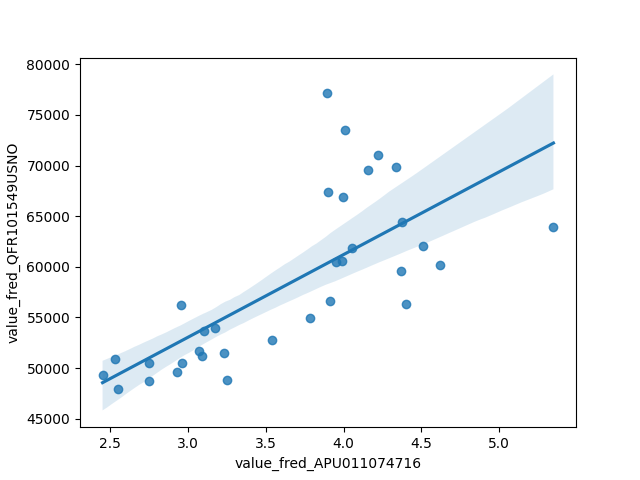
\includegraphics[scale = 0.9]{plots/plot_2026-09-06.png}
\caption{Raw Regression Plot for 2026-09-06}
\end{figure}
\newpage
\subsection{Detrended Regression}
\noindent Regresses the residuals of each series after removing its own linear time trend, so a shared trend can no longer drive the result on its own. A relationship that stays significant here is better evidence of a genuine link between the two series.

\begin{center}
\begin{tabular}{lclc}
\toprule
\textbf{Dep. Variable:}                       & value\_fred\_QFR101549USNO\_detrended & \textbf{  R-squared:         } &     0.137   \\
\textbf{Model:}                               &                  OLS                  & \textbf{  Adj. R-squared:    } &     0.109   \\
\textbf{Method:}                              &             Least Squares             & \textbf{  F-statistic:       } &     4.928   \\
\textbf{Date:}                                &            Sun, 06 Sep 2026           & \textbf{  Prob (F-statistic):} &   0.0339    \\
\textbf{Time:}                                &                14:30:55               & \textbf{  Log-Likelihood:    } &   -323.18   \\
\textbf{No. Observations:}                    &                     33                & \textbf{  AIC:               } &     650.4   \\
\textbf{Df Residuals:}                        &                     31                & \textbf{  BIC:               } &     653.4   \\
\textbf{Df Model:}                            &                      1                & \textbf{                     } &             \\
\textbf{Covariance Type:}                     &               nonrobust               & \textbf{                     } &             \\
\bottomrule
\end{tabular}
\begin{tabular}{lcccccc}
                                              & \textbf{coef} & \textbf{std err} & \textbf{t} & \textbf{P$> |$t$|$} & \textbf{[0.025} & \textbf{0.975]}  \\
\midrule
\textbf{const}                                &   -1.542e-09  &      778.512     & -1.98e-12  &         1.000        &    -1587.786    &     1587.786     \\
\textbf{value\_fred\_APU011074716\_detrended} &    3391.3160  &     1527.650     &     2.220  &         0.034        &      275.654    &     6506.978     \\
\bottomrule
\end{tabular}
\begin{tabular}{lclc}
\textbf{Omnibus:}       &  1.706 & \textbf{  Durbin-Watson:     } &    0.705  \\
\textbf{Prob(Omnibus):} &  0.426 & \textbf{  Jarque-Bera (JB):  } &    1.192  \\
\textbf{Skew:}          &  0.465 & \textbf{  Prob(JB):          } &    0.551  \\
\textbf{Kurtosis:}      &  2.962 & \textbf{  Cond. No.          } &     1.96  \\
\bottomrule
\end{tabular}
%\caption{OLS Regression Results}
\end{center}

Notes: \newline
 [1] Standard Errors assume that the covariance matrix of the errors is correctly specified.

\begin{figure}
\centering
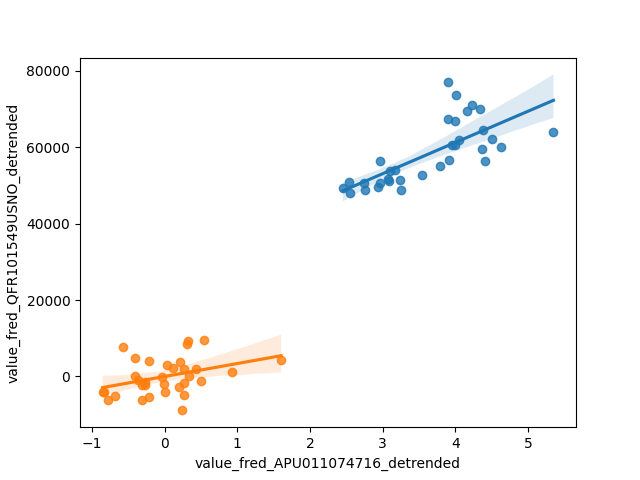
\includegraphics[scale = 0.9]{plots/plot_2026-09-06_detrended.png}
\caption{Detrended Regression Plot for 2026-09-06}
\end{figure}
\newpage
